\documentclass{article}
\usepackage[utf8]{inputenc}
\usepackage{hyperref}

\title{Assignment01}
\author{Shin Dong-Ha}
\date{September 2018}

\usepackage{graphicx}

\begin{document}


\maketitle

\section{What is GIT?}
Before use git, I should know what GIT is, and when I should use it. Shortly, GIT is a program of helping you to manage your own program and it has many functions to do it such as remembering source code of your program's previous version, or add up the new version of source code with previous code to update program and so on. And if you use GITHUB (\url{https://github.com/}) whoever you allowed can change your source code wherever the internet works so if you work not in a static space, and work with your team members(even if you work solo GIT and GITHUB will be helpful too) I strongly recommend to use GIT and GITHUB.


\section{How I Use GIT}
When I first heard about the GIT was when I was sophomore. I tried to make a website with my friend using 'python' and 'django'. We had to work in team and then we needed to use some code sharing program. And we found the program GIT so we could work in team. After that, when I became junior I had to do a team project and we used GIT again. It was my first start of using GIT.

Then we had to know how to use GIT. As I said first, GIT has version control function and this function is the main function of GIT so let's start with it.

To make GIT manage our source codes, we had to tell GIT where is the source codes are. We call this location 'repository'. Below is the way to create your repository.

\newpage

\begin{figure}[h]
\centering
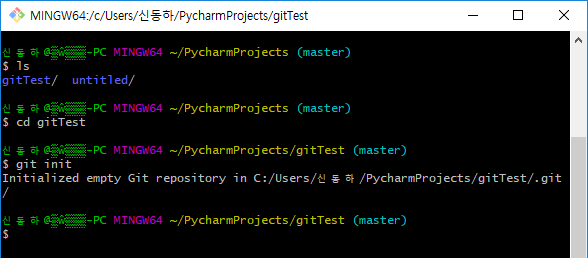
\includegraphics[scale=0.75]{init.png}
\caption{creating repository}
\label{fig:creating repository}
\end{figure}

I first moved into the folder where I want to make repository(cd gitTest). And then typed 'git init'. Then the git shows me the sentence 'initialized empty Git repository in ~' and created the folder '.git' so the GIT can recognize this folder is used as a repository. As we made a repository, we can add some source codes to here. Let's do it.
\begin{figure}[h]
\centering
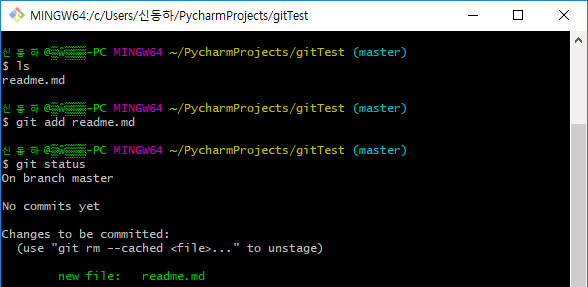
\includegraphics[scale=0.75]{add.png}
\caption{adding file to the repository}
\label{fig:adding file to the repository}
\end{figure}

I made the file readme.md before and typed 'git add readme.md', 'git status' then GIT shows the sentence "~... new file: readme.md'. It means that GIT recognized the file readme.md and ready to update the git repository with that readme.md file. So let's really update the version of my 'gitTest' repository. We call it 'commit'
\begin{figure}[h]
\centering
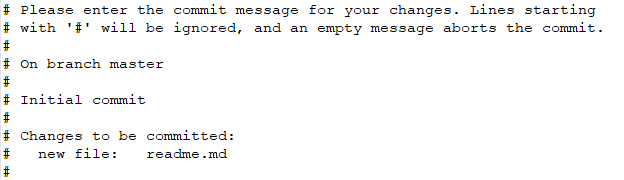
\includegraphics[scale=0.73]{commit_message.png}
\caption{writing commit message}
\label{fig:writing commit message}
\end{figure}

After you type 'git commit' the text editor comes out and have you to write the commit message. You can write the commit message from the first blank line to describe what changes were made in this commit.
\begin{figure}[h]
\centering
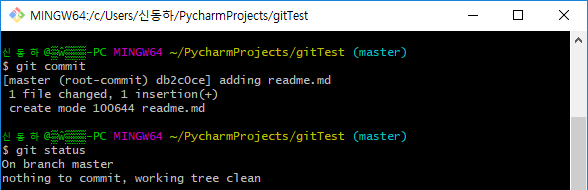
\includegraphics[scale=0.75]{commit.png}
\caption{committing file to the repository}
\label{fig:committing file to the repository}
\end{figure}

After you write commit message and save that file, commit is done and shows the message 'working tree clean'. If you want to modify that 'readme.md' file, then you should do again from 'adding file to the repository' with chanaged file. But at someday you may want to remove your committed files, in that case we should do 'remove' the file from the repository. At this time, we will remove only from the git repository not from our hard disk.
\begin{figure}[h]
\centering

\includegraphics[scale=0.75]{remove.png}
\caption{removing file from the repository}
\label{fig:removing file from the repository}
\end{figure}

After you type 'git rm --cached readme.md' GIT shows you the message rm 'readme.md' Now the GIT no more manages the file readme.md

Finally let's use GITHUB. To use GITHUB, we should log in and make new repository.
\newpage
\begin{figure}[h]
\centering
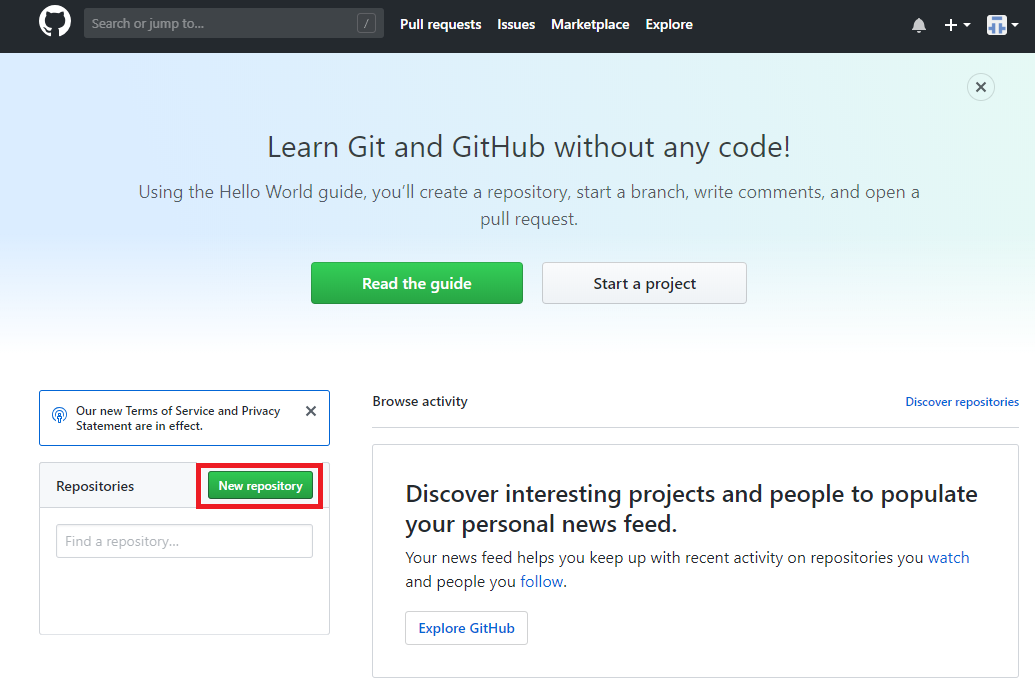
\includegraphics[scale=0.42]{GITHUB.png}
\caption{making new repository from the GITHUB}
\label{fig:making new repository from the GITHUB}
\end{figure}

\begin{figure}[h]
\centering
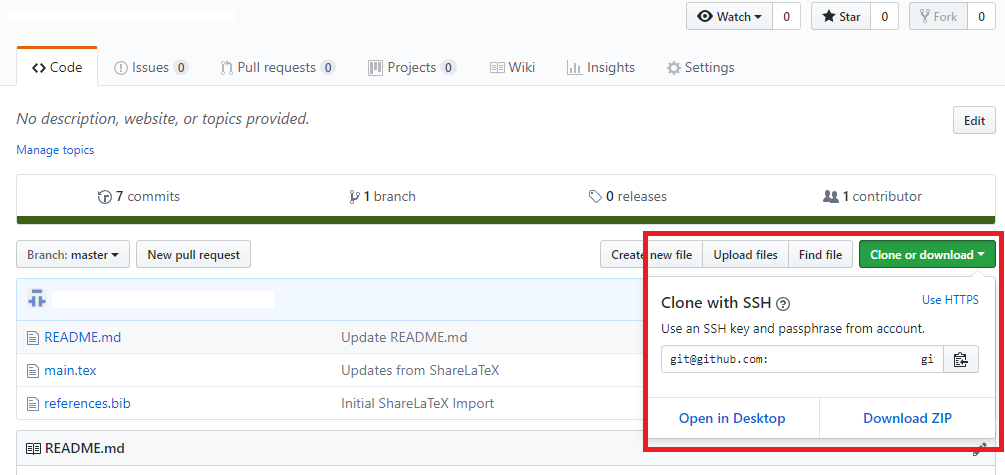
\includegraphics[scale=0.42]{ssh.png}
\caption{copying ssh to clone the repository}
\label{fig:copying ssh to clone the repository}
\end{figure}

\begin{figure}[h]
\centering
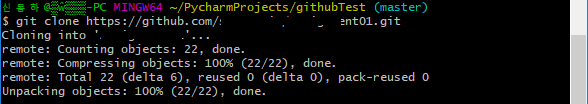
\includegraphics[scale=0.75]{clone.png}
\caption{cloning online repository to the local computer}
\label{fig:cloning online repository to the local computer}
\end{figure}
\newpage
After you create new repository, then you can find clone button at the right side.
Just copy the ssh or https and paste it to the git like below.
Now the online repository is cloned to your computer. Use it for you!
\section{Conclusion}
I showed you where and how to use the GIT and GITHUB. While doing team projects or other developing projects this will be used very frequently. So know more about GIT will be helpful to be in a computer engineer, scientist.
\end{document}
